\section{Super Resolution}

\subsection{Data}
\begin{frame}{Data}
    \small
    \begin{itemize}
        \item 在制作数据集时, 对比不同源遥感影像超分, 不需要准备哨兵影像, 只需高分影像
        \item 高分影像多光谱(低分)和融合多光谱全色后的影像(高分)可用于超分影像对的制作
        \item 多光谱全色融合影像可当作高分辨率影像使用吗?(纹理+颜色)
    \end{itemize}
\end{frame}

\subsection{Method}
\begin{frame}{Deep learning Model}
    \small
    现阶段的初步想法是
    \begin{itemize}
        \item SRCNN
        \item SRGAN
        \item SRResCGAN
    \end{itemize}
    
\end{frame}

% \begin{frame}{可用哨兵数据空间位置}
%     \small
%     考虑到六幅影像的范围有重叠, 只用其中一组即可
%     \begin{figure}
%         \centering
%         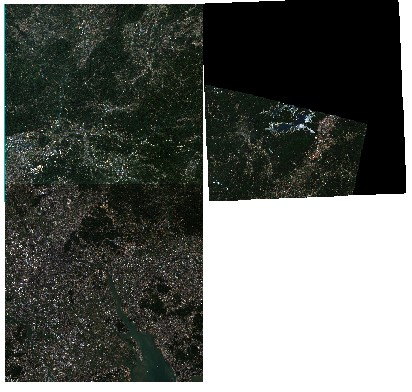
\includegraphics[width=6cm]{pic/pic0115.jpg}
%         \caption{哨兵可用重叠}
%         \label{fig:0109}
%     \end{figure}
% \end{frame}

% \begin{frame}{数据查询}
%     \begin{columns}
%         \column{0.3\textwidth}
%         \begin{itemize}
%             \item \small{对广东区域进行影像检索}
%         \end{itemize}

%         \column{0.7\textwidth}
%         \begin{figure}
%             \centering
%             % Requires \usepackage{graphicx}
%             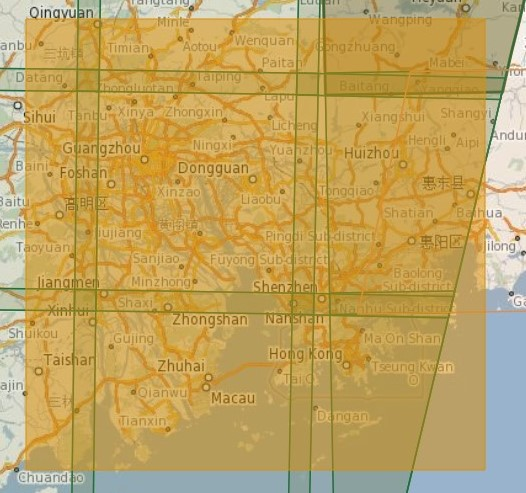
\includegraphics[width=5cm]{pic/pic0101.jpg}
%             \caption{影像查询地区}
%             \label{fig:0101}
%         \end{figure}
%     \end{columns}
% \end{frame}